\documentclass{article}
\usepackage{graphicx}
\usepackage{amsmath}
\usepackage{amssymb}
\usepackage[T1]{fontenc}
\usepackage[polish]{babel}
\usepackage[utf8]{inputenc}
\title{Lista 1 Zadanie 3}
\author{Marcin Zubrzycki}
\begin{document}
\maketitle
\section{Treść Zadania}
Należy skonstruować automaty skończone równoważne z następującymi wyrażeniami regularnymi:
\begin{itemize}
  \item $10+(0+11)0*1$
  \item $01[((10)*+111)*+0]*1$
  \item $((0+1)(0+1))*+((0+1)(0+1)(0+1))*$
\end{itemize}
\section{Rozwiązanie}
\begin{figure}[h]
  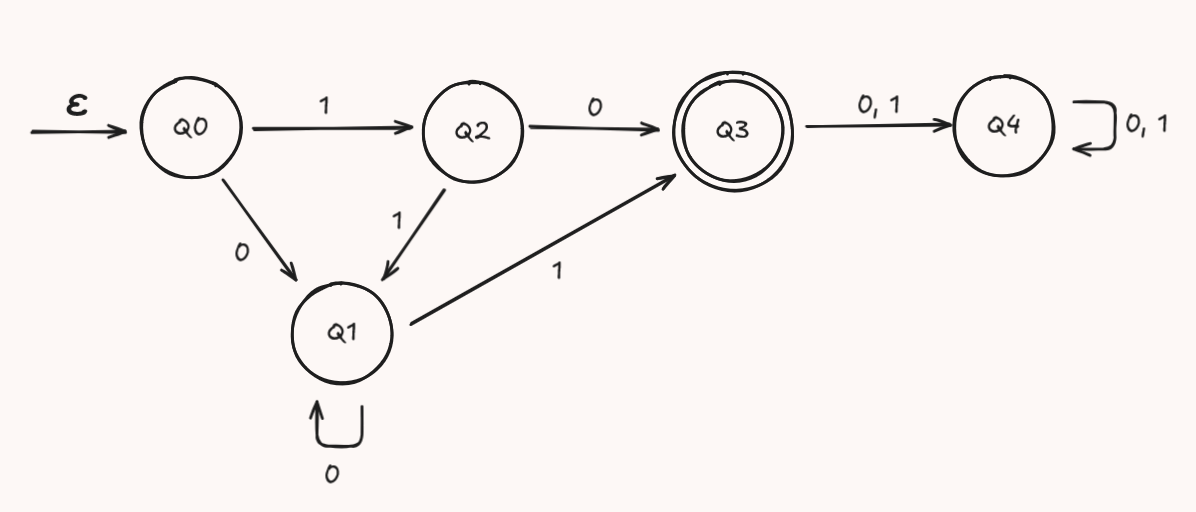
\includegraphics[width=1\textwidth]{11.png}
  \caption{DFA dla podpunktu 1}
\end{figure}
\begin{figure}[h]
  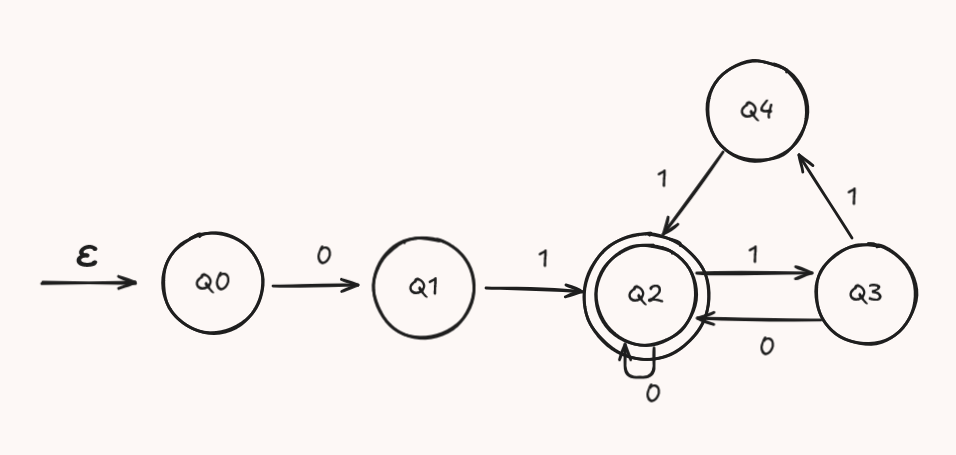
\includegraphics[width=1\textwidth]{12.png}
  \caption{NFA dla podpunktu 2}
\end{figure}
\begin{figure}[h]
  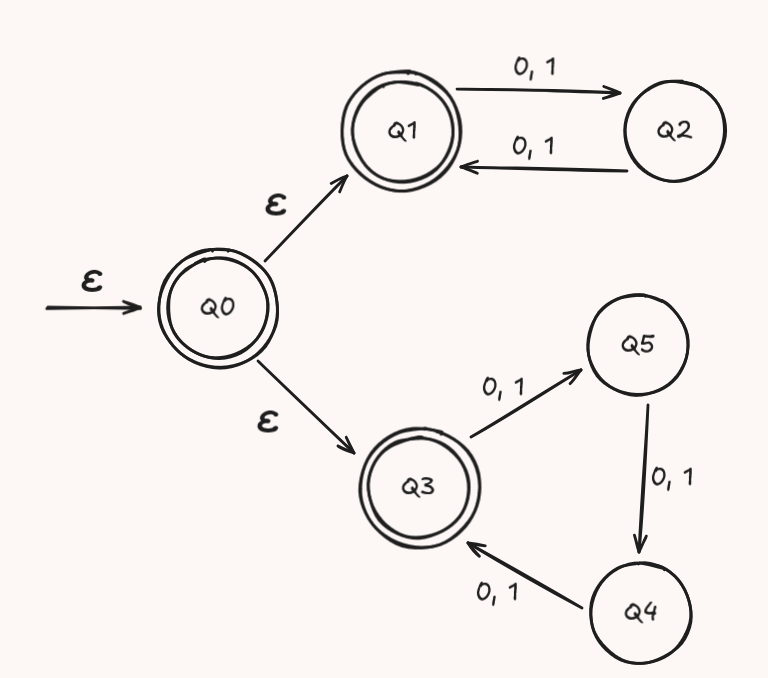
\includegraphics[width=1\textwidth]{13.png}
  \caption{NFA-$\varepsilon$ dla podpunktu 3}
\end{figure}
\subsection{Język pierwszy}
Język składa się ze słów które na początku mają $0$ lub $11$, potem dowolną ilość $0$ i kończą się dokładnie jednym $1$. Dodatkowo w skład języka wchodzi również słowo $w = 10$.
Słowo $w = 10$ jest akceptowane przez automat M. Pozostałe słowa muszą zaczynać się od $0$ lub $11$, obie drogi prowadzą do stanu $Q0$ w którym w pętli można przetworzyć dowolną liczbę zer i dokładnie jedną jedynką przejść do stanu akceptującego $Q3$, z którego można
jedynie wyjść, odrzucając wszystkie słowa które nie kończą się dokładnie jedną jedynką. $L(M) = 10+(0+11)0*1$
\subsection{Język drugi}
Język składa się ze słów zaczynających się od znaków $01$, potem zawierającą dowolną ilość powtórzeń $10$, $111$ lub $0$ i finalnie kończących się dokładnie jedną jedynką.
Automat M przyjmuje do stanu $Q2$ jedynie słowa z odpowiednim prefiksem, następnie pozwala odbyć odpowiednią pętle po napotkaniu powtarzającego się podsłowa. $10: Q2 \rightarrow Q3\rightarrow Q2$, $111: Q2 \rightarrow Q3 \rightarrow Q4 \rightarrow Q2$ i $0: Q2 \rightarrow Q2$
Każda skuteczna pętla kończy się w stanie $Q2$ z którego można przetworzyć jedną $1$ aby skończyć w stanie akceptującym.  $L(M) = 01[((10)*+111)*+0]*1$
\subsection{Język trzeci}
Język składa się ze słów długości $\ell$ spełniającą $\ell = 2n \lor \ell = 3n$ dla $n \in \mathbb{Z}$. Automat M pozwala wyjść ze stanu $Q0$ do pętli trójstanowej lub dwustanowej, która kończy w stanie akceptującym po każdej pełnej iteracji. $L(M) = ((0+1)(0+1))*+((0+1)(0+1)(0+1))*$
\end{document}